\documentclass[10pt]{article}
\usepackage{graphicx}
\usepackage{subcaption}
\usepackage[T1]{fontenc}
\usepackage{amsmath}
\usepackage{lipsum}
\usepackage{hyperref}
\usepackage[utf8]{inputenc}
\usepackage[letterpaper,margin=1in]{geometry}
\usepackage[parfill]{parskip}
\usepackage[europeanresistors, american]{circuitikz}
\usetikzlibrary{arrows,shapes,calc,positioning}
\usetikzlibrary{shapes}
\usetikzlibrary{plotmarks}

\newcommand{\oscope}[2] % #1 = name , #2 = rotation angle
{
    \draw[thick,rotate=#2] (#1) circle (12pt)
    (#1) ++(-0.35,-0.1) -- ++(0.3,0.3) --++(0,-0.3)-- ++(0.3,0.3) --++(0,-0.3);
}

\begin{document}

\title{\textbf{\Large{\textsc{ECE320:} Fields and Waves}} \\ \Large{Lab 1 Report: Waves on Transmission Lines}}
\author{Alp Tarım, Pranshu Malik}

\maketitle

\section{Introduction}

This laboratory focused on investigating the characteristics of transmission lines, studying voltage and current 
propagation along them, as well as its depedance on the nature of load impedance.


\section[Determining the Characteristic Impedance, Z0]{Determining the Characteristic Impedance, {$Z_0$}}

We varied the load on the switch box until we saw little or no traces of reflected waves.
This was at $Z_L = 50 \Omega$ which is also equal to the charactertic impedance 
since we know that the reflections nullify when $Z_L = Z_0$. The corresponding waveforms
captured at the generator input (channel 1, top) and the transmission line input (channel 2, bottom) 
are shown in Figure 1.

\begin{figure}[h]
    \centering
    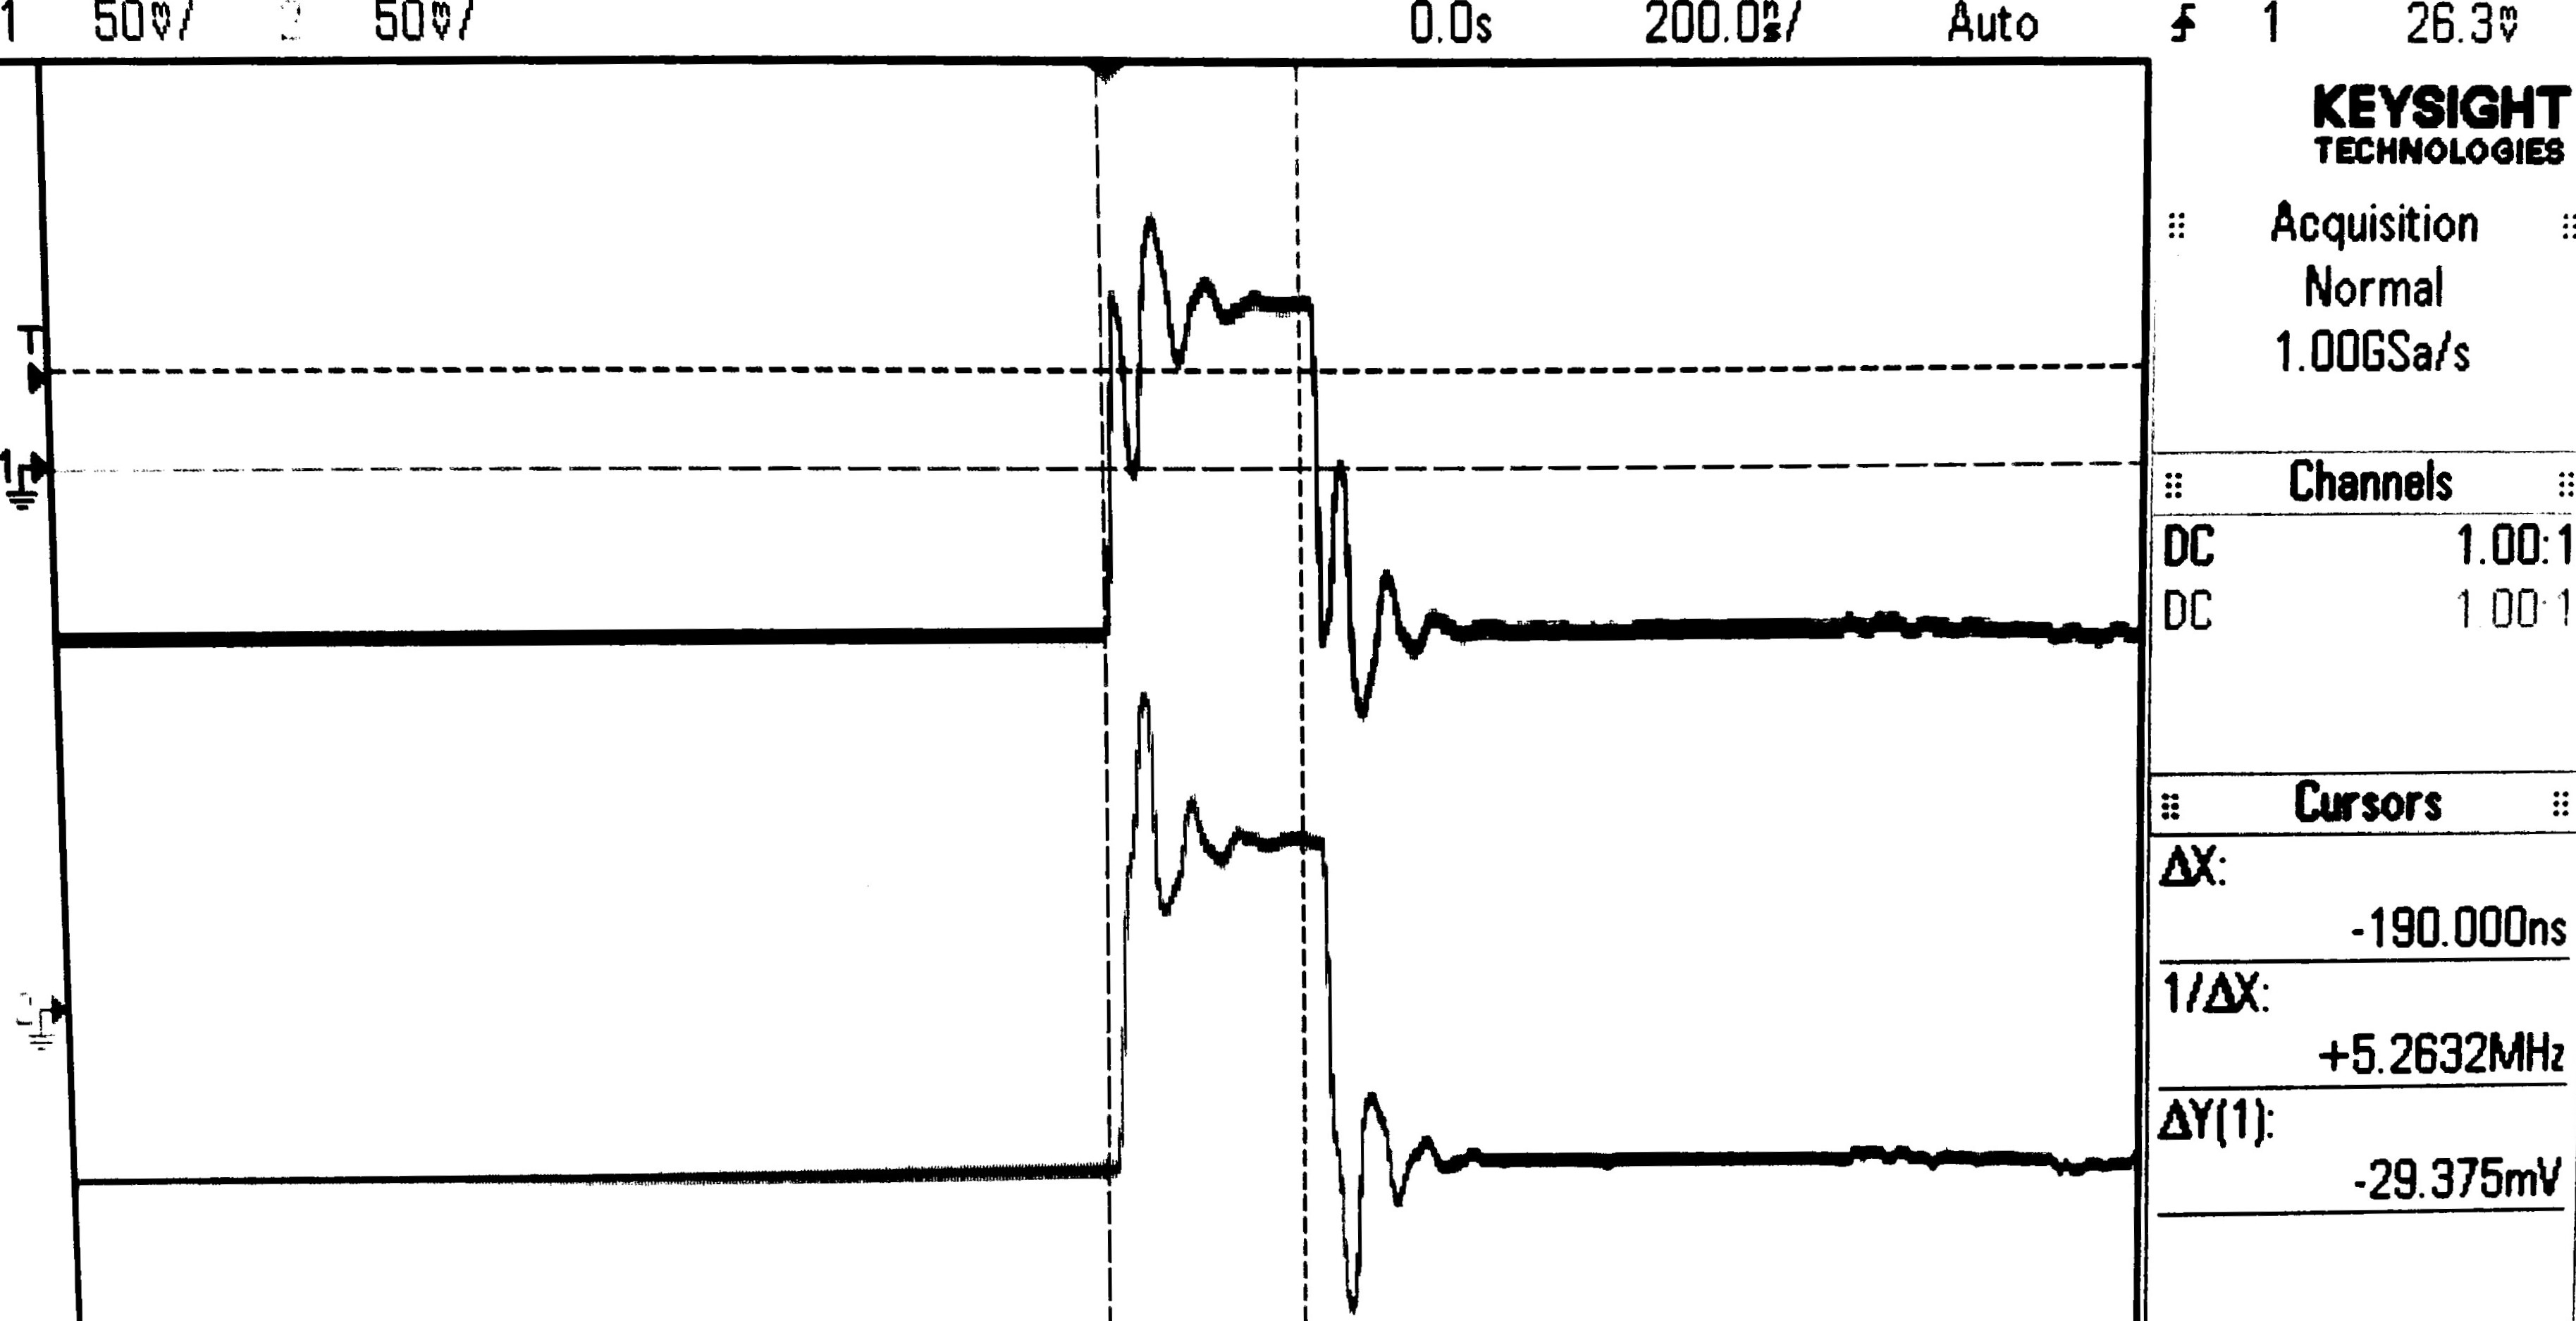
\includegraphics[width=6.54cm]{../photos/lab1/load_matched.jpg}
    \caption{Transmission line terminated with load equal to $Z_0$}
    \label{tline_matching_z_0}
\end{figure}


\section[Determining Z0 using V/I]{Determining $Z_0$ using $\frac{\tilde V^+(z=0)}{\tilde I^+(z=0)}$}

\begin{figure}[!hb] \centering
    \begin{circuitikz} 
        \draw
        (0,2) to [sqV, l_=$\tilde V_g$] (0, 0) -- (2,0)
        to [tline, l_=Transmission Line, o-o] (7,0)
        to [R, l=$Z_L$] (7, 2)
        to [tline, l=${Z_0, \beta, L}$, o-o] (2,2)
        to [R, l_=$Z_g$, i<^=$\tilde I$] (0, 2);
        
        \draw (2,2.35) node{$\tilde V$} (2, 2);
        \draw (2,0) -- (2.5,-0.15) to[sV, l_=\footnotesize{CH1}, color=white, name=CH1] (2.5,1.75) -- (2, 2);
        \oscope{CH1}{0}
        \draw (7,0) -- (8,-0.15) to[sV, l_=\footnotesize{CH2}, color=white, name=CH2] (8,1.75) -- (7, 2);
        \oscope{CH2}{0}
        \draw (0,0) to[short, *-*] node[ground]{} (0,0);
        \draw [dotted] (2,-0.35) -- (2,0.35) (7,-0.35) -- (7,0.35)
        (2, -0.5) node{$z=0$} (2, -0.35) (7, -0.5) node{$z=L$} (7, -0.35);
    \end{circuitikz}
    \caption{Laborartory setup for studying characteristcs of tranmission lines}
    \label{tline_diag}
\end{figure}

As seen in the picture the voltage at $v_g$ is 154mV and $v_1$ is equal to 51mV. Assuming the resistance in between is $100\Omega$ 
$i_l$ = $\frac{0.154-0.051}{100}$ = $1.03*10^-3$A. Which means $Z_0=\frac{v_1}{i_l}=\frac{0.051}{1.03*10^-3}=49.51\Omega~50\Omega $

\begin{figure}[h] \centering
    \begin{circuitikz} 
        \draw [dotted][thick] (0,0) -- (0,2) (2,0) -- (2,2) (0, 2) -- (-1, 2) (2, 2) -- (3, 2);
        \draw (0,1.5) to [R, l=$R_{\text{shunt}}$, i>^=$\tilde I$, *-*] (2, 1.5);
        \draw (0,0.15) -- (2, 0.15);
        \draw (1, 0.15) to [short, *-*] node[ground]{} (1,0.15);
        \draw (0,0.15) circle (1.5pt);
        \draw (2,0.15) circle (1.5pt);
        \draw (2,0.15) -- (2.5,-0.15) to[sV, l_=$\tilde V_2$, color=white, name=CH2] (2.5,1.35) -- (2, 1.5);
        \oscope{CH2}{0}
        \draw (0,0.15) -- (-0.5,-0.15) to[sV, l=$\tilde V_1$, color=white, name=CH1] (-0.5,1.35) -- (0, 1.5);
        \oscope{CH1}{0}

        \draw (4.75,1) node[]{$\displaystyle{\tilde I = \frac{\tilde V_1 - \tilde V_2}{R_{\text{shunt}}}}$} (4.75,1);
    \end{circuitikz}
    \caption{Estimating input current through a shunt resistance}
    \label{shunt_diag}
\end{figure}

Thus, we can see something there. We know that $\tilde V_2 = \tilde V(z=0)$ and thus, we can confirm the
value of $Z_0$ through the following relation: $\frac{\tilde V^+(z=0)}{\tilde I^+(z=0)}$.

\section{Observation of Travelling Waves}

We observed the following waveforms at different points, C = 0m, D = 30m, E = 60m, F = 90m along the 

\begin{figure} [h]
    \centering
    \begin{subfigure}[b]{0.35\textwidth}
        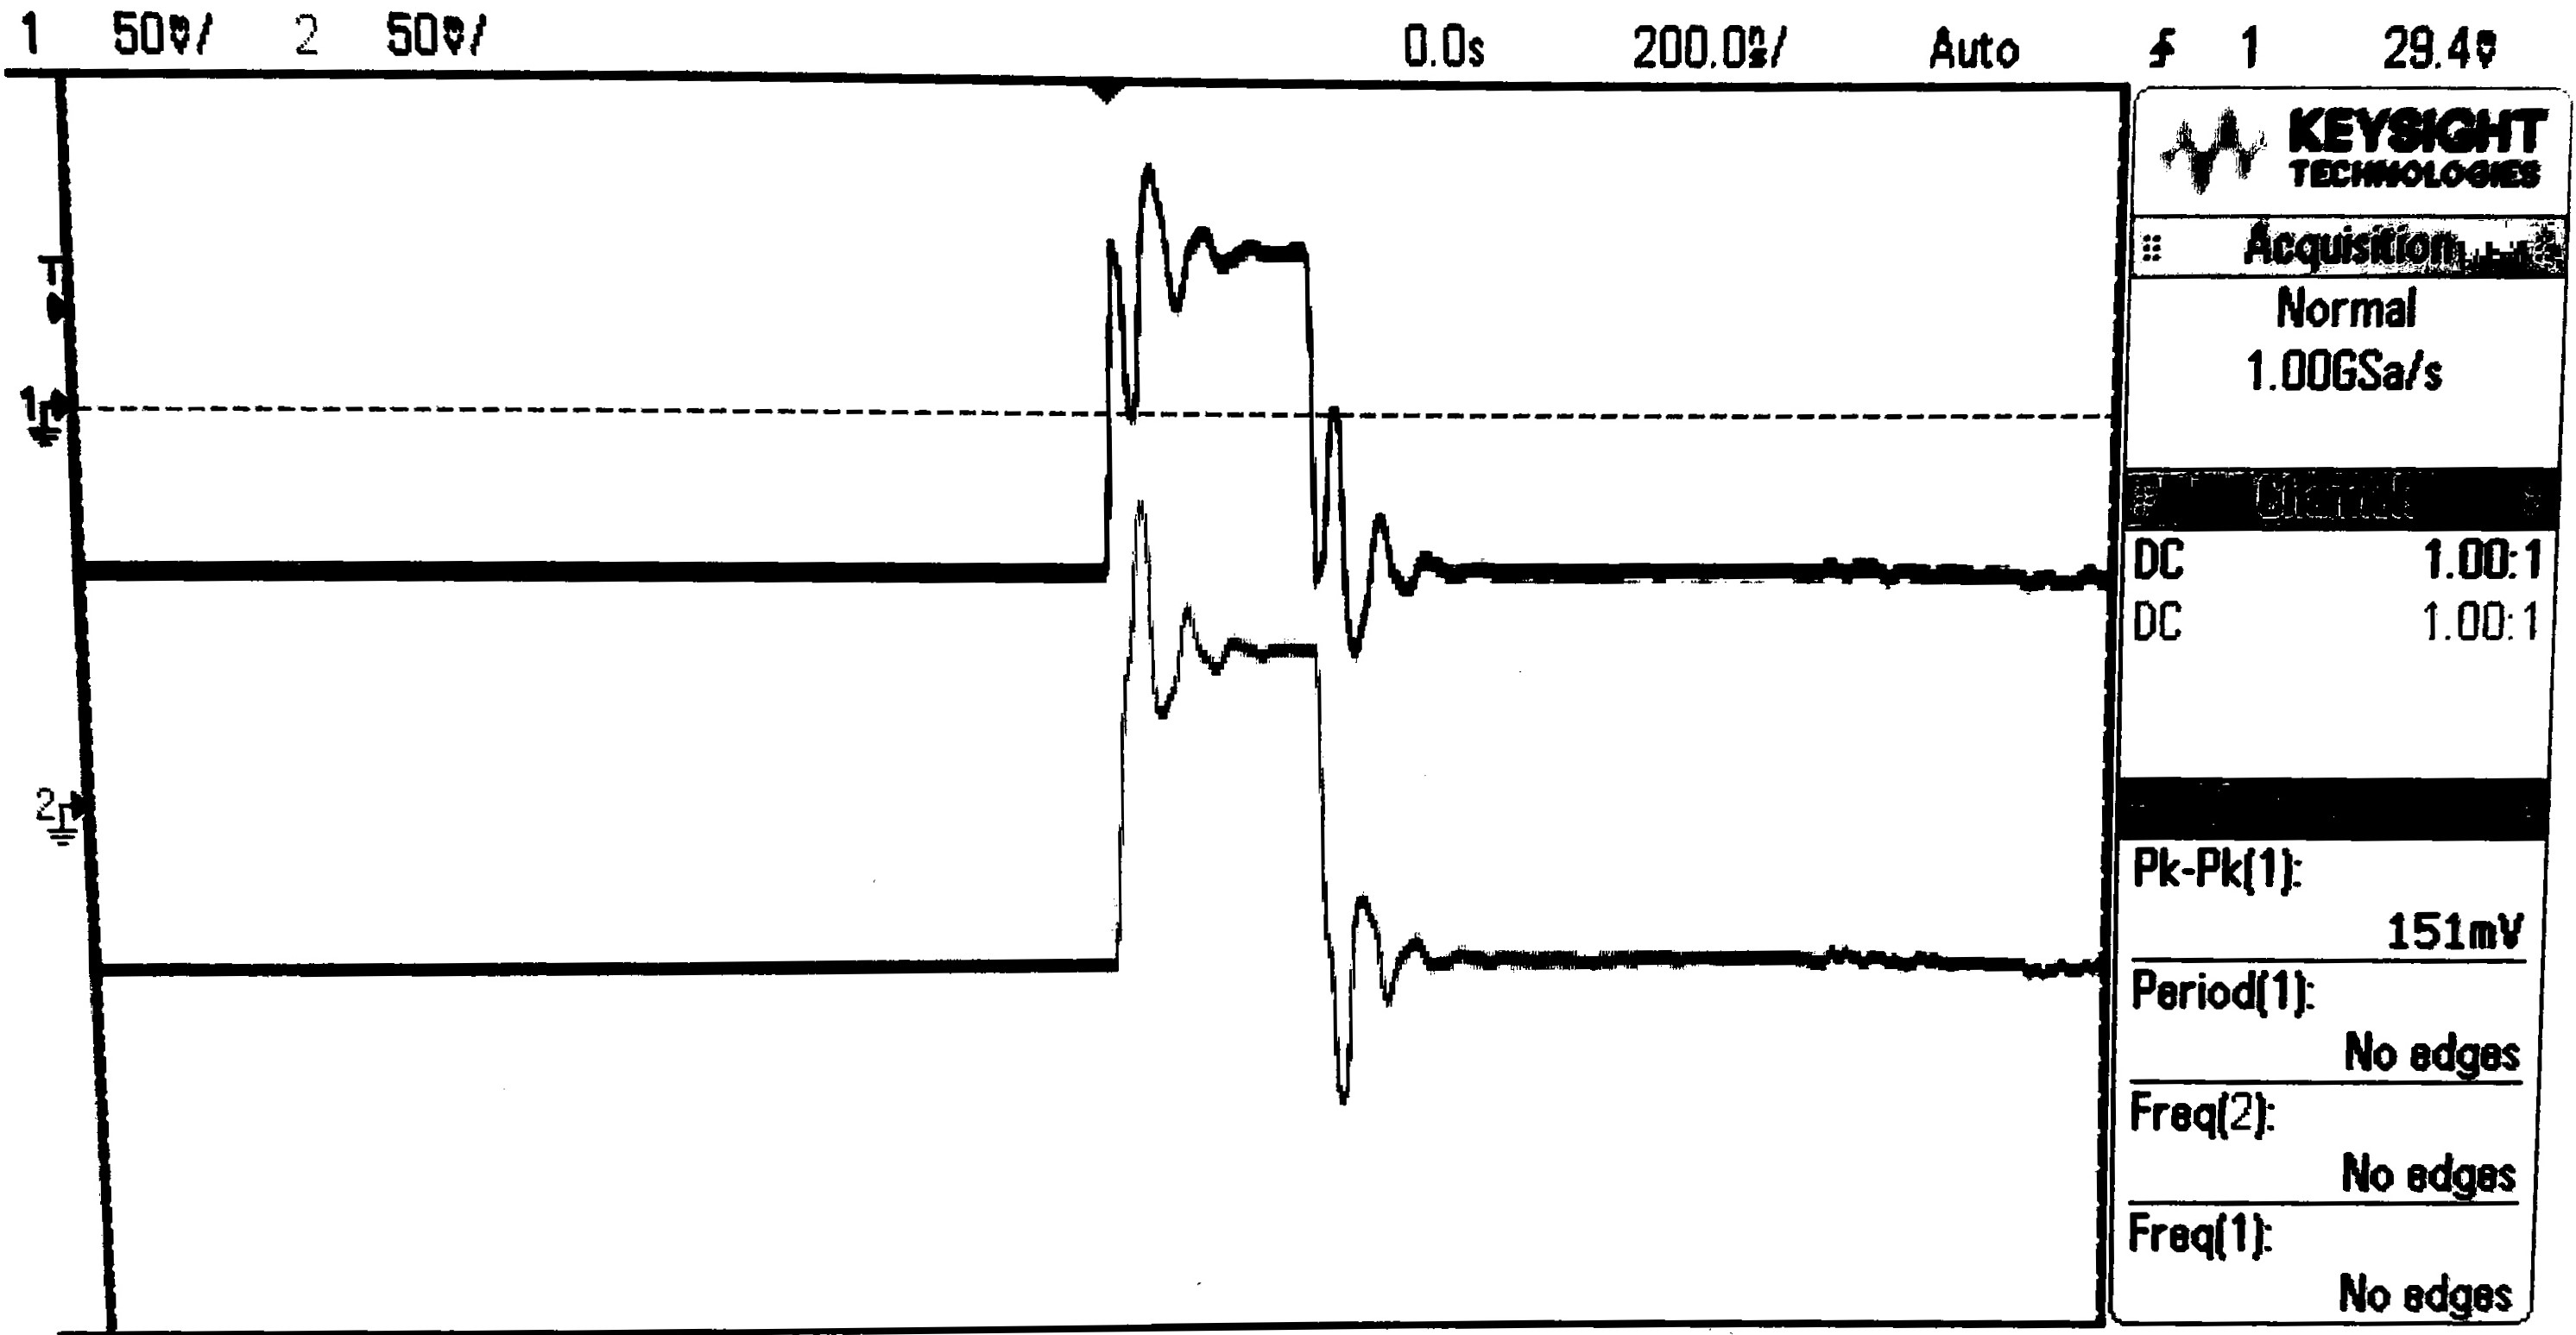
\includegraphics[width=\textwidth]{../photos/lab1/v_t_pt_c.jpg}
        \caption{Point C}
    \end{subfigure}
    \begin{subfigure}[b]{0.35\textwidth}
        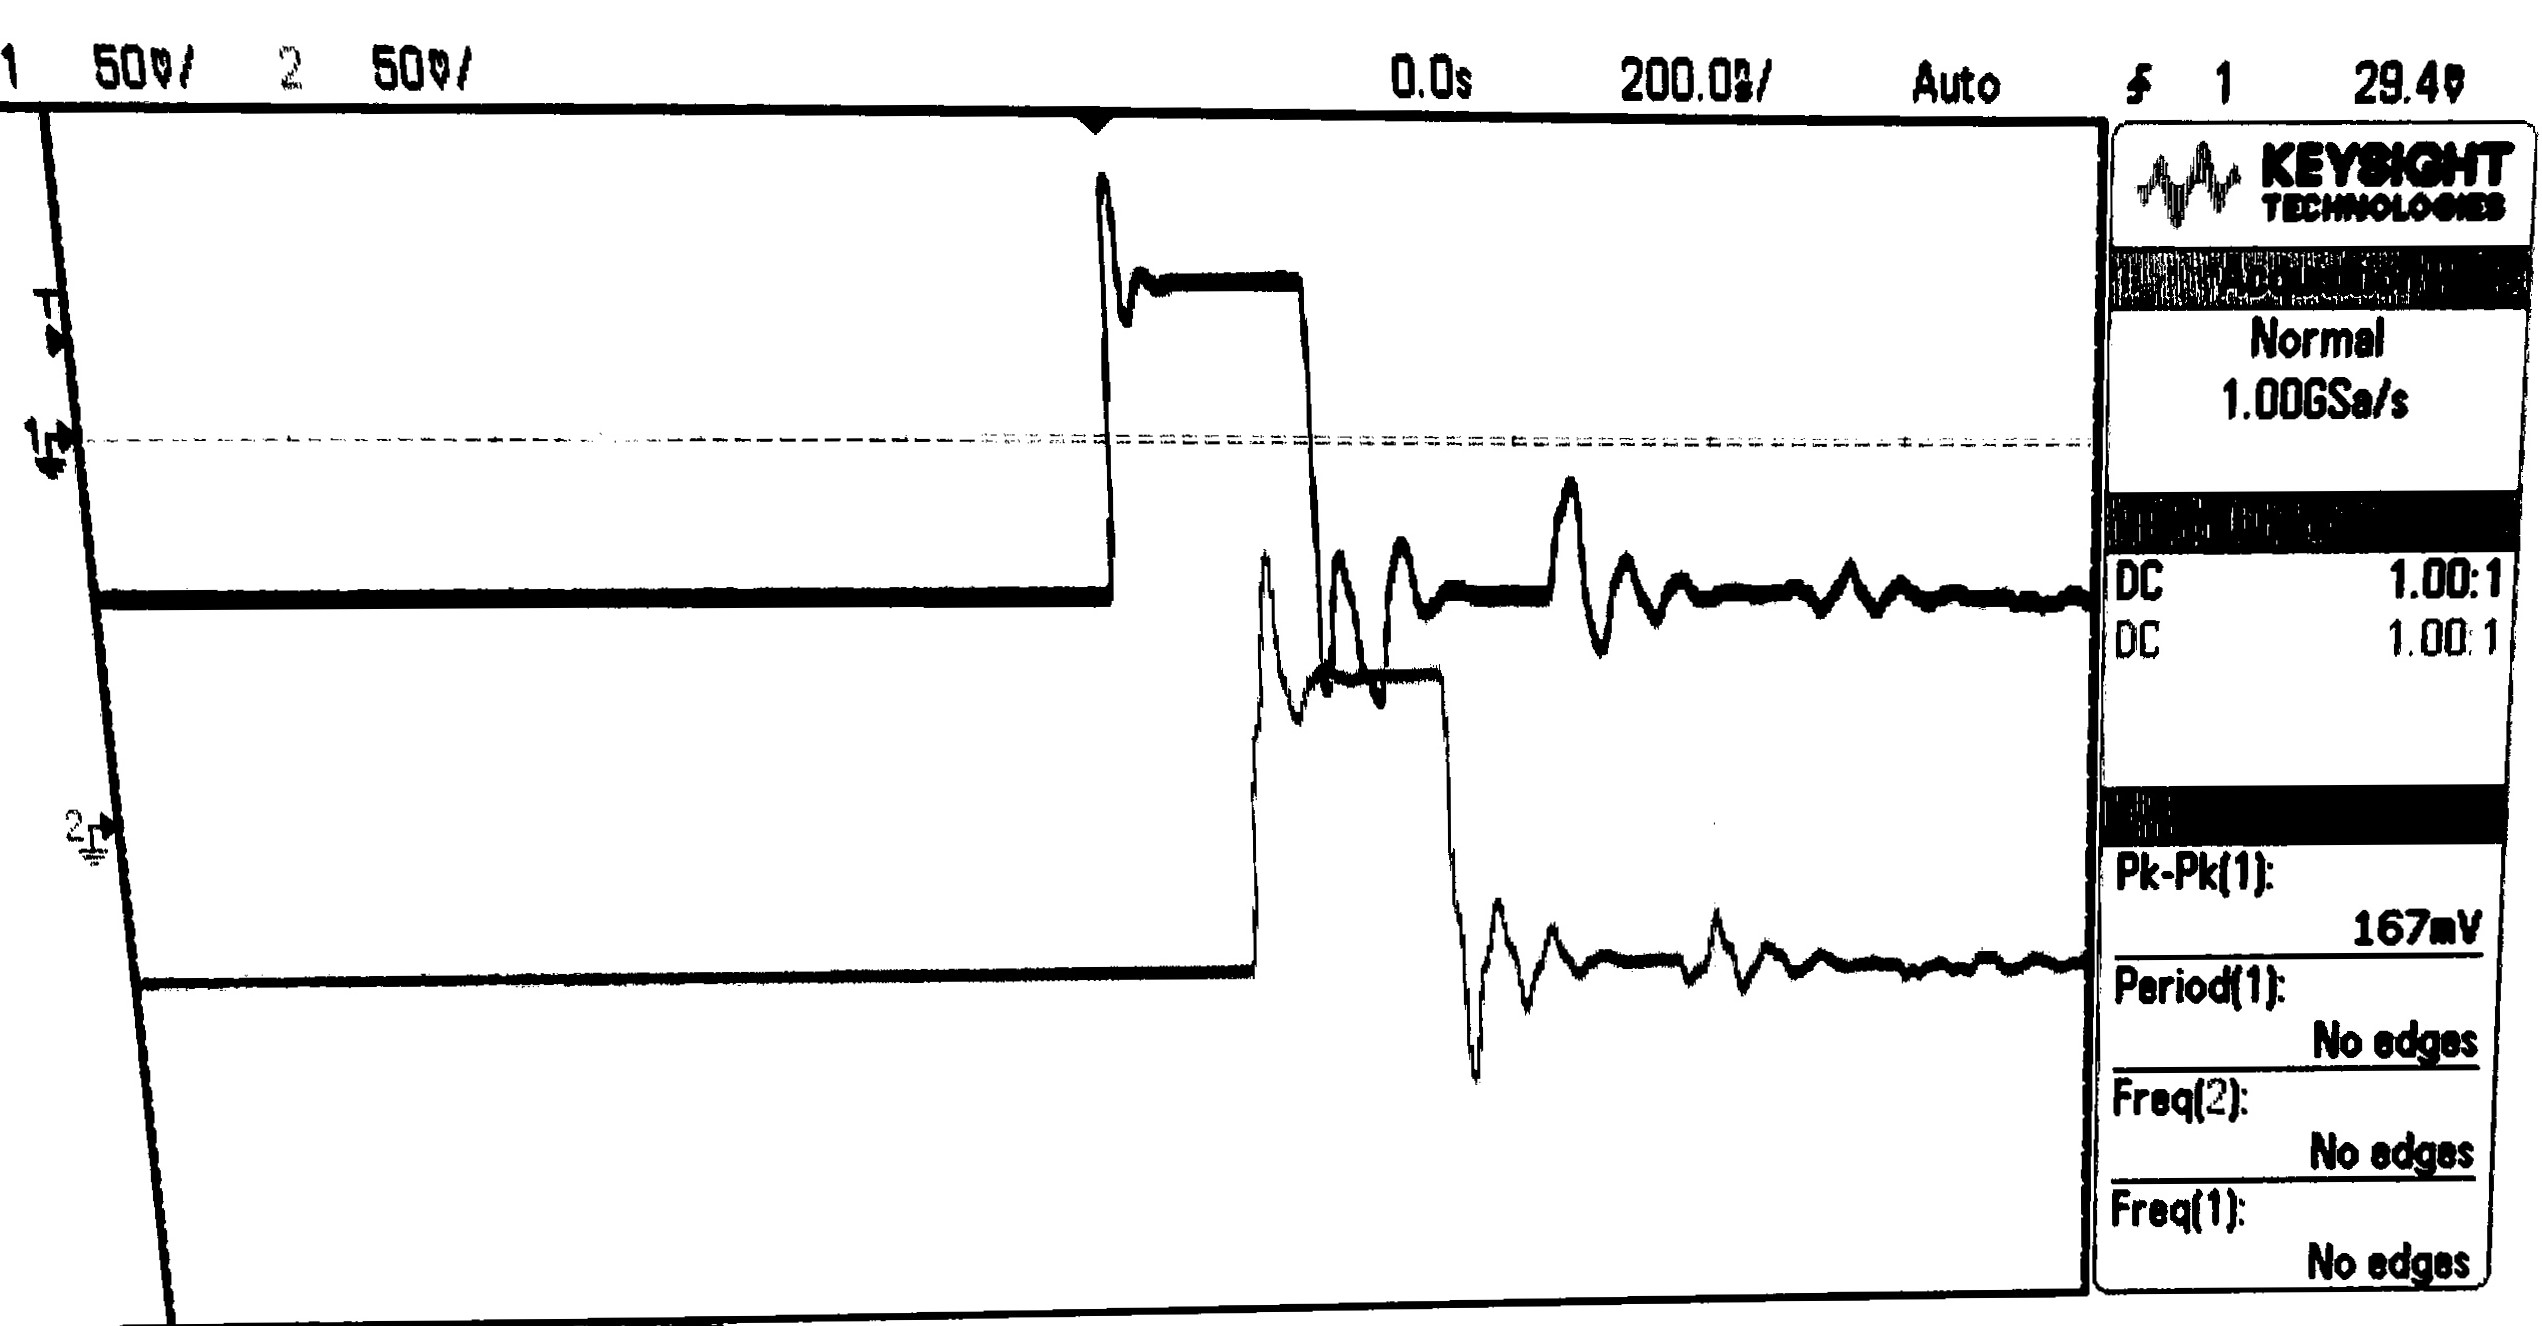
\includegraphics[width=\textwidth]{../photos/lab1/v_t_pt_d.jpg}
        \caption{Point D}
    \end{subfigure}
    \begin{subfigure}[b]{0.35\textwidth}
        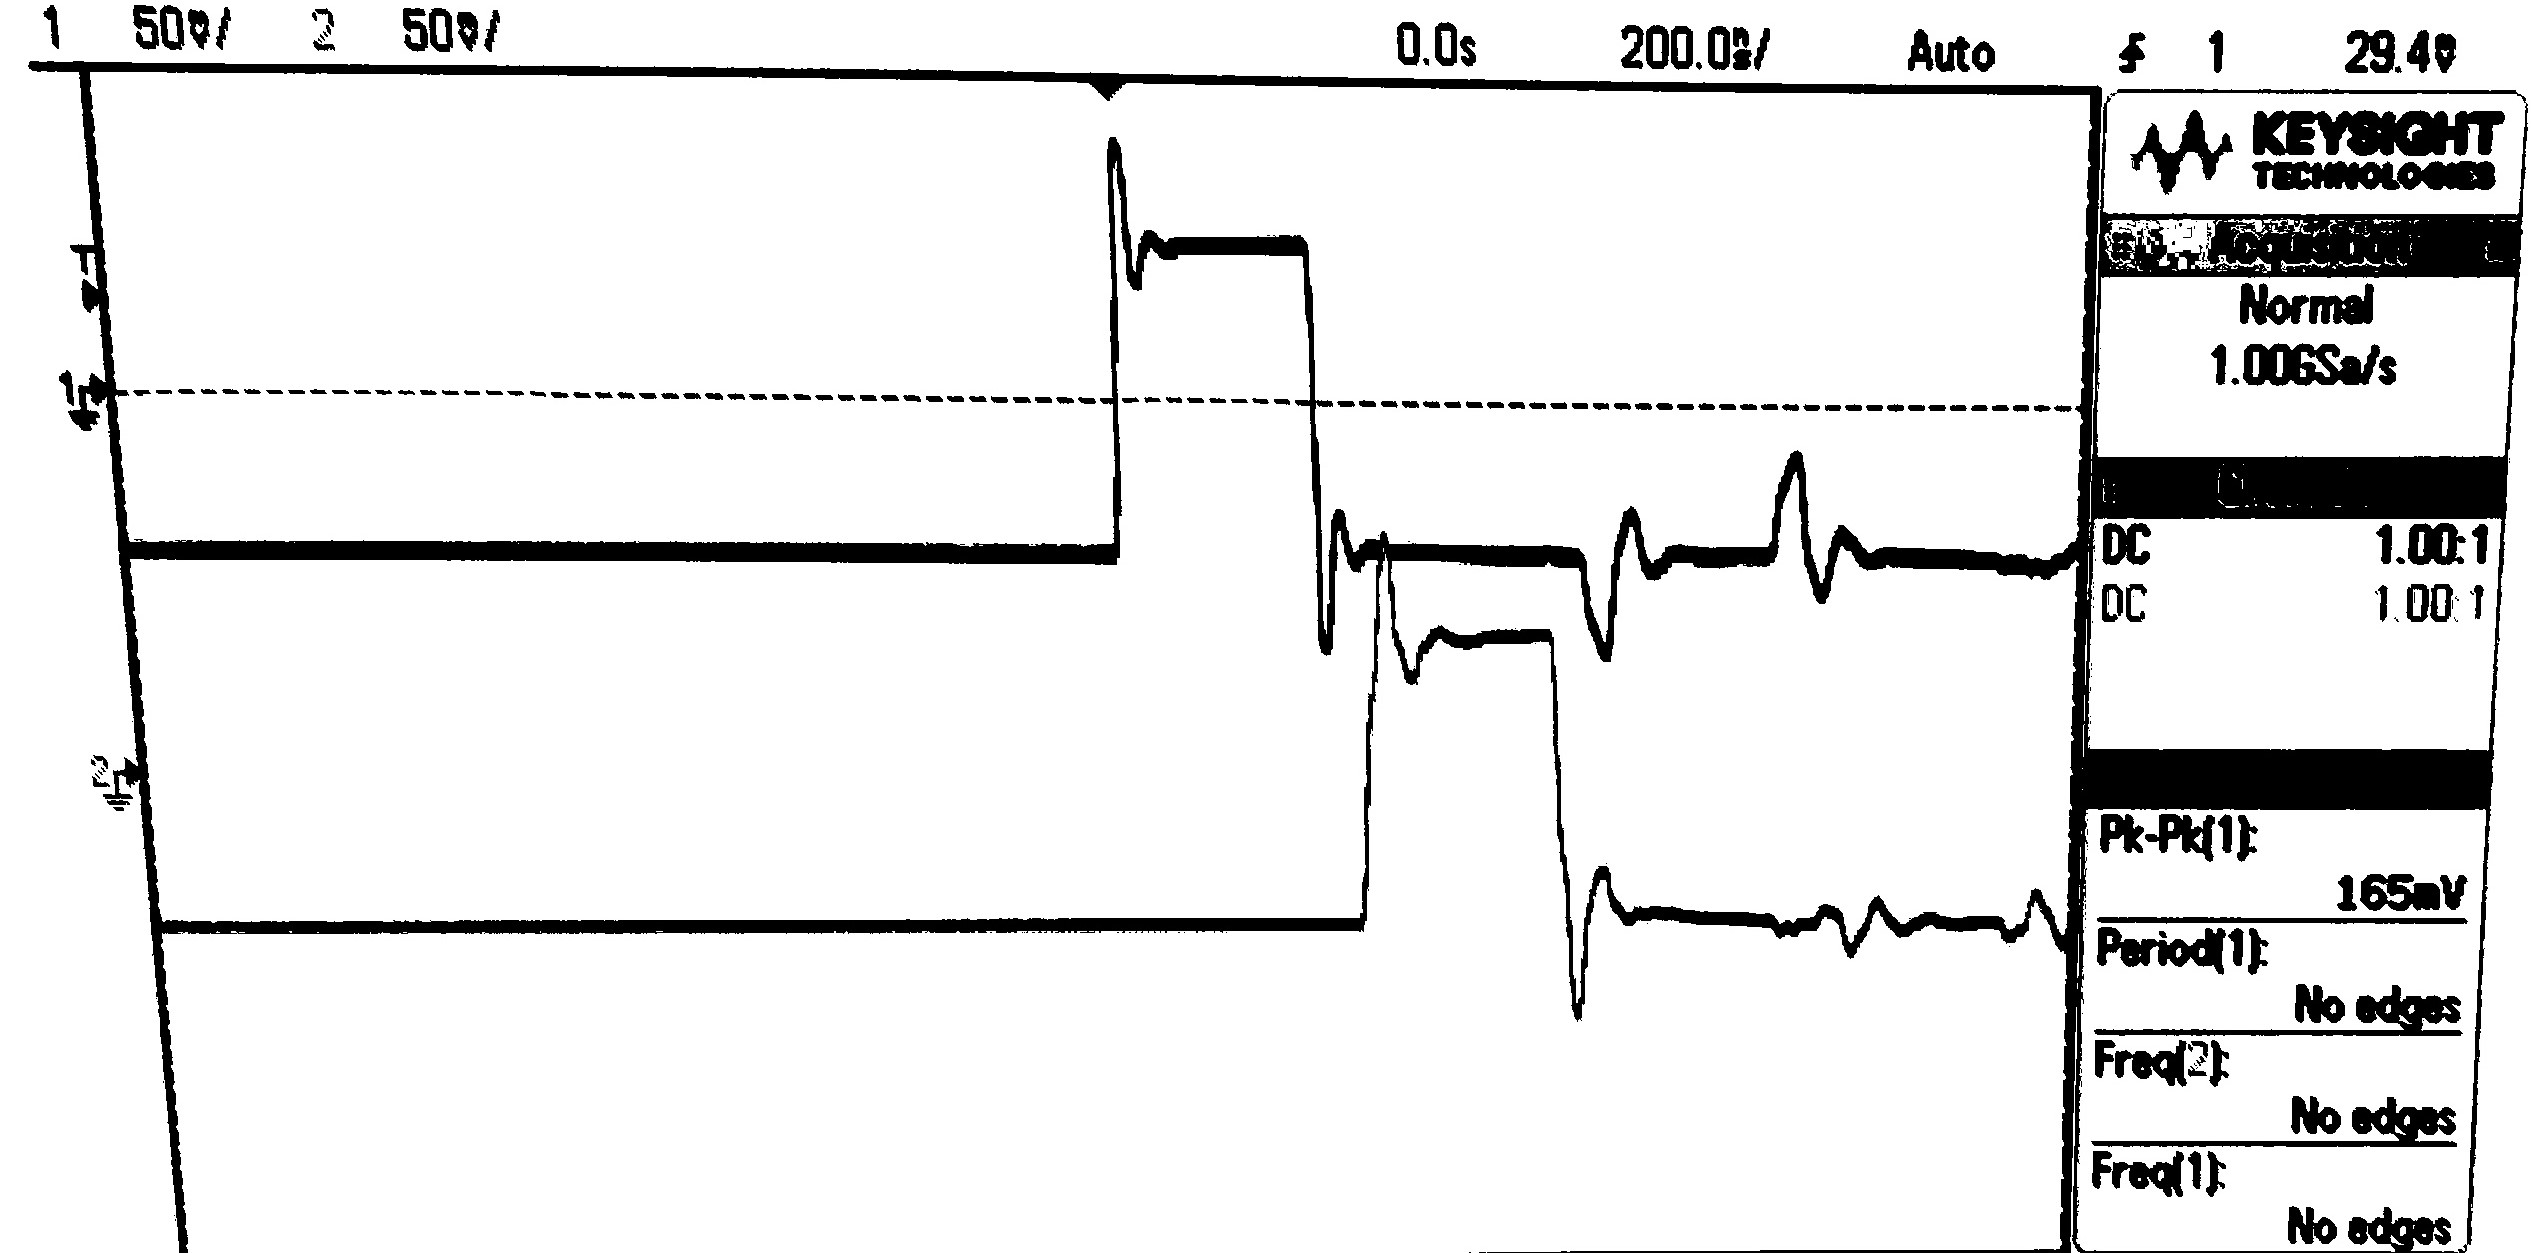
\includegraphics[width=\textwidth]{../photos/lab1/v_t_pt_e.jpg}
        \caption{Point E}
    \end{subfigure}
    \begin{subfigure}[b]{0.35\textwidth}
        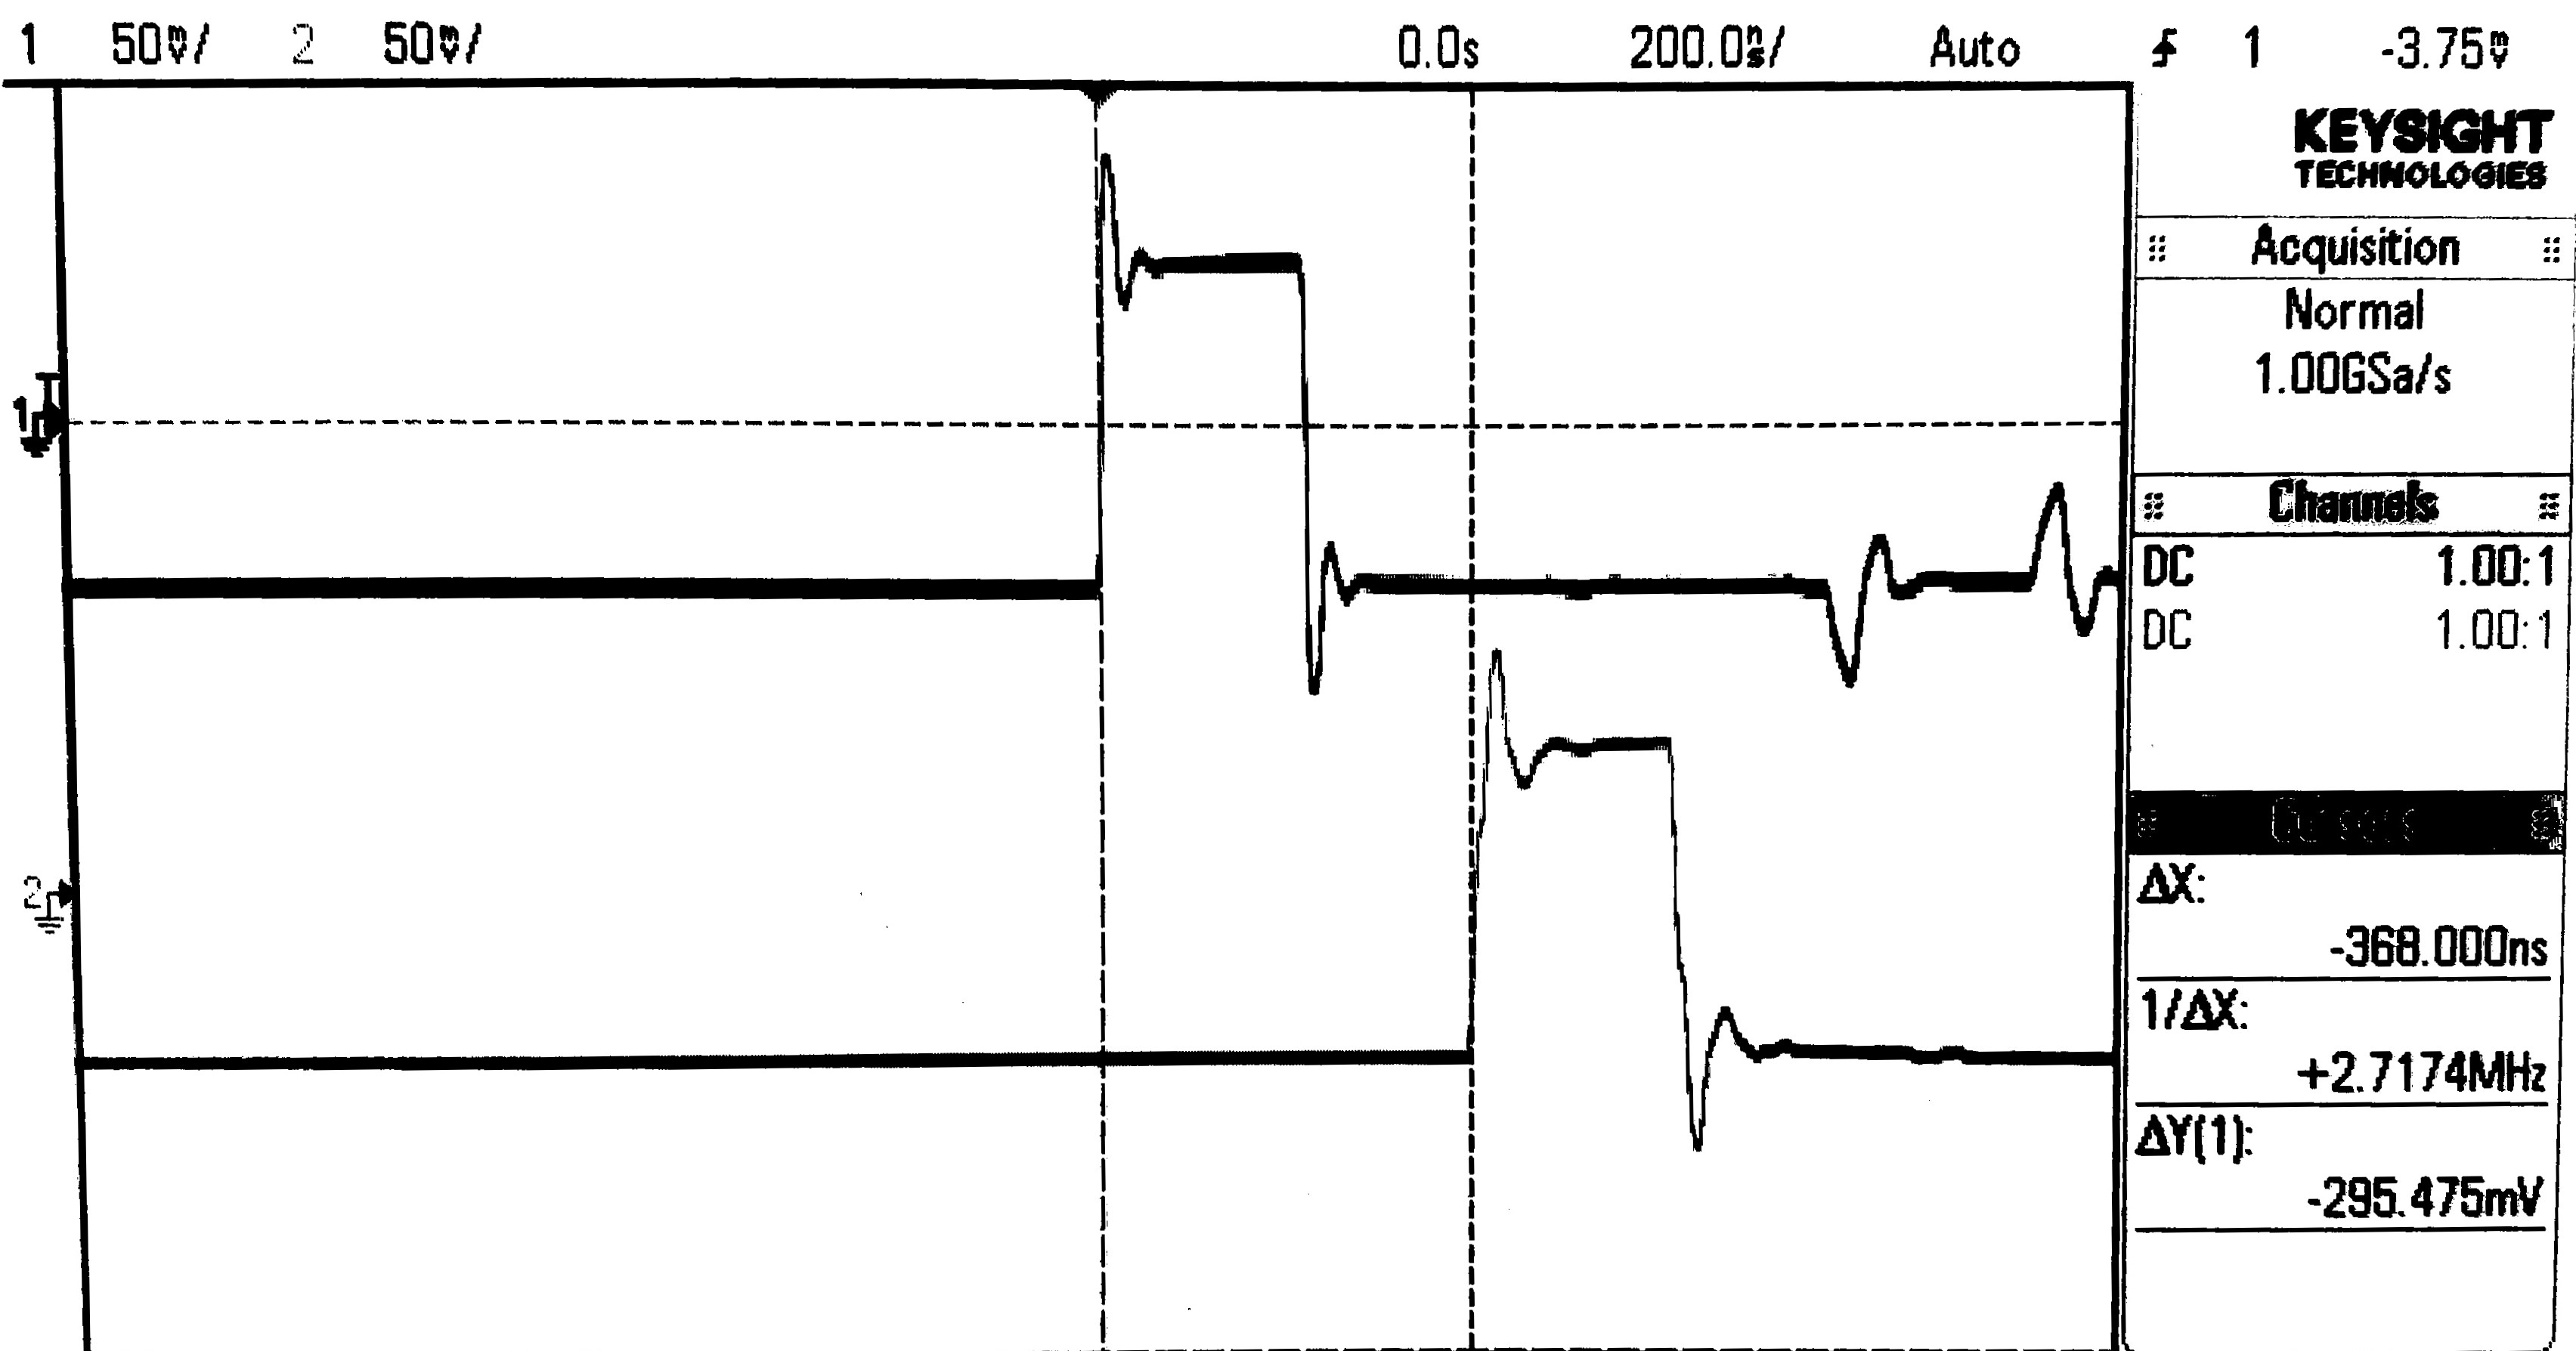
\includegraphics[width=\textwidth]{../photos/lab1/v_t_pt_f.jpg}
        \caption{Point F}
    \end{subfigure}
    \caption{Observed waveforms, $V(t)$, at different loactions along the transmission line}
    \label{}
\end{figure}

The table of delays are:

\begin{table} [h]
    \[
        \begin{array}{c|c}
            \textbf{Point} & \Delta t \textbf{ (ns)} \\ \hline
            \text{D} & 130\\
            \text{E} & 244\\
            \text{F} & 368
        \end{array}
    \]
    \caption{Time delay for pulses}
\end{table}

\section{Determination of Velocity of Propagation}

The velocity of propagation of the signal can be calculated by the relation $v_p = \frac{\Delta L}{\Delta t}$, given that
we are able to track the same point on the waveform at both places. Using the data from table 1,
we get that the average velocity of propagation is $v_{p, \text{avg}} = 2.44 \cdot 10^8 \text{m/s}$.

We know that the phase velocity of an electromagentic wave in space with magnetic permeability, $\mu$,
and electric permittivitty, $\epsilon$  is given by: 

\[
    v_p = \frac{1}{\sqrt{\mu \epsilon}}
\]

\section{Simple Reflection}

We know that

\section{Multiple Reflections}


\section{Input Impedance and Transmission Line Length}

\begin{figure}[h] \centering
    \begin{circuitikz} 
        \draw
        (0, 2) to [V, l_=$\tilde V_g$] (0, 0) -- (2, 0)
        to [R, l_=${Z_{\text{in}}}$, -*] (2, 2)
        to [R, l_=$Z_g$] (0, 2);

        \draw (2, 2) -- (2.25, 2.25);
        
        \draw 
        (3.45, 2.4) 
        node[]{$\displaystyle{\tilde V_{\text{in}} = \tilde V_g\frac{Z_{\text{in}}}{Z_{\text{in}} + Z_g}}$} 
        (3.45, 2.4);
    \end{circuitikz}
    \caption{Voltage division over net input impedance, $Z_\text{in}$}
    \label{volt_diag}
\end{figure}

We know that the impedance changes.

\[
    Z_{\text{in}} = Z_0 \frac{1+\Gamma_d}{1-\Gamma_d} = Z_0 \frac{Z_0 + jZ_L\tan{\beta L}}{Z_L + jZ_0\tan{\beta L}}
\]

\section{Conclusion}

Lorem ipsum dolor sit amet, consectetur adipisicing elit, sed do eiusmod tempor
incididunt ut labore et dolore magna aliqua. Ut enim ad minim veniam, quis
nostrud exercitation ullamco laboris nisi ut aliquip ex ea commodo consequat.
Duis aute irure dolor in reprehenderit in voluptate velit esse cillum dolore eu
fugiat nulla pariatur.

\section{Notes}

All pictures taken during the lab were post-processed in a batch using a custom script
that bit-wise inverted the pixels and the thresholded to produce a binarized image. No
adjustments or modifications were made to the readings, for which the oscilloscope's measurements
are also shown alongside the waveforms. All work can be found at 
\href{https://github.com/pranshumalik14/ece320-labs}{\texttt{github.com/pranshumalik14/ece320-labs}}.

\end{document}